Una red neuronal convolucional (CNN) es un tipo de red neuronal artificial que se distingue por incluir una o más capas convolucionales, donde se realiza la operación matemática de convolución. Este tipo de red ha encontrado una amplia aplicación en el campo de la visión artificial. Surgidas de los estudios sobre la corteza visual del cerebro, estas redes han demostrado un éxito notable en el reconocimiento de imágenes.


A pesar de su origen vinculado principalmente al procesamiento visual, las CNN también han mostrado efectividad en la clasificación de documentos. Según \cite{goldberg2016primer} en A Primer on Neural Network Models for Natural Language Processing, las redes neuronales convolucionales son eficaces en la clasificación de documentos porque tienen la capacidad de identificar características sobresalientes (como tokens o secuencias de tokens). Esto resulta útil para tareas de clasificación donde se espera encontrar pistas locales sólidas sobre la pertenencia a una clase, independientemente de que estas pistas puedan presentarse en diversas partes de la entrada. En la Figura \ref{fig:an9} se puede apreciar a una red neuronal convolucional con una matriz bidimensional de tamaño 7x5 donde cada fila representa a cada elemento en la oración de entrada, la tarea de esta red convolucional es extraer frases útiles para realizar una clasificación binaria que indique el sentimiento de la oración de un fragmento de texto.
\begin{figure}[h!]
	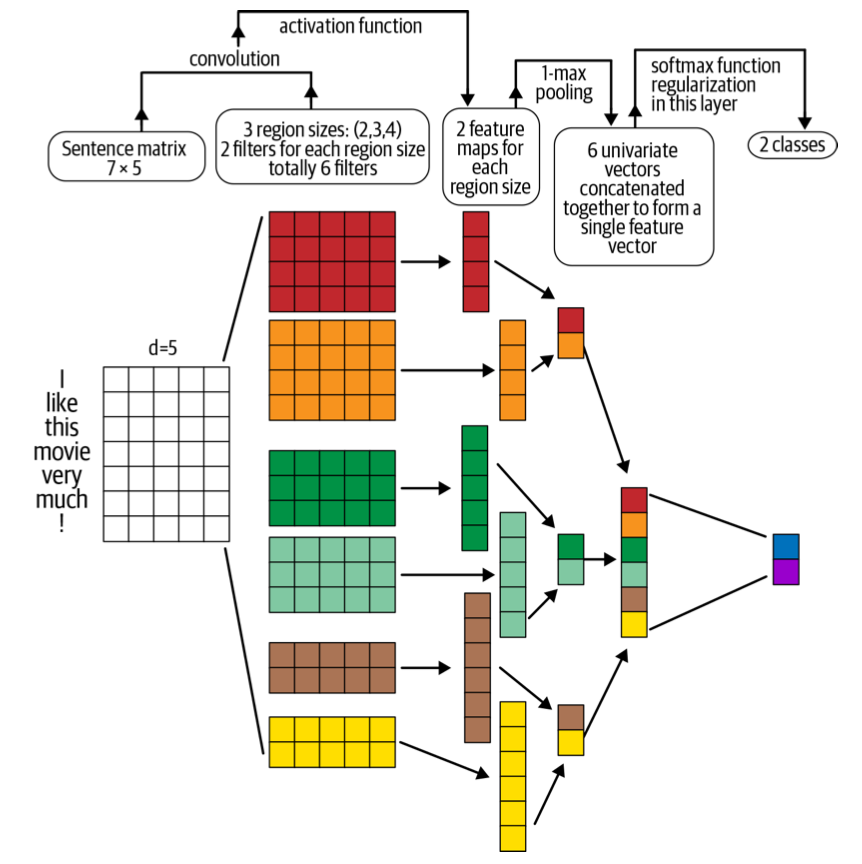
\includegraphics[width=0.6\textwidth]{capitulo2/figuras/an9.png}
	\caption[Modelo CNN en accion]{Modelo CNN en accion
		\\\textit{Fuente: Extraído de} \protect\cite[p. 25]{vajjala2020practical}}
	\label{fig:an9}
\end{figure}

La arquitectura básica de una CNN incluye capas de convolución, las cuales aplican filtros para extraer rasgos relevantes de la entrada. También se incorporan capas de agrupación (pooling) para reducir el tamaño de las representaciones, manteniendo las características más importantes. Por último, las capas totalmente conectadas se encargan de la clasificación final, basándose en los rasgos extraídos por las capas anteriores. Esta arquitectura básica se modifica para adaptarse al procesamiento y clasificación de texto.

